\documentclass[runningheads,a4paper,11pt]{report}

\usepackage{algorithmic}
\usepackage{algorithm} 
\usepackage{array}
\usepackage{amsmath}
\usepackage{amsfonts}
\usepackage{amssymb}
\usepackage{amsthm}
\usepackage{caption}
\usepackage{comment} 
\usepackage{epsfig} 
\usepackage{fancyhdr}
\usepackage[T1]{fontenc}
\usepackage{geometry} 
\usepackage{graphicx}
\usepackage[colorlinks]{hyperref} 
\usepackage[latin1]{inputenc}
\usepackage{multicol}
\usepackage{multirow} 
\usepackage{rotating}
\usepackage{setspace}
\usepackage{subfigure}
\usepackage{url}
\usepackage{verbatim}
\usepackage{xcolor}

\geometry{a4paper,top=3cm,left=2cm,right=2cm,bottom=3cm}

\pagestyle{fancy}
\fancyhf{}
\fancyhead[LE,RO]{Sense}
\fancyhead[RE,LO]{Bogdan-Daniel B\u{a}l\u{a}nescu}
\fancyfoot[RE,LO]{ITSG 2019-2020}
\fancyfoot[LE,RO]{\thepage}

\renewcommand{\headrulewidth}{2pt}
\renewcommand{\footrulewidth}{1pt}
\renewcommand{\headrule}{\hbox to\headwidth{%
  \color{lime}\leaders\hrule height \headrulewidth\hfill}}
\renewcommand{\footrule}{\hbox to\headwidth{%
  \color{lime}\leaders\hrule height \footrulewidth\hfill}}

\hypersetup{
pdftitle={artTitle},
pdfauthor={name},
pdfkeywords={pdf, latex, tex, ps2pdf, dvipdfm, pdflatex},
bookmarksnumbered,
pdfstartview={FitH},
urlcolor=cyan,
colorlinks=true,
linkcolor=red,
citecolor=green,
}
% \pagestyle{plain}

\setcounter{secnumdepth}{3}
\setcounter{tocdepth}{3}

\linespread{1}

% \pagestyle{myheadings}

\makeindex


\begin{document}

\begin{titlepage}
\sloppy
\begin{center}
BABE\c S BOLYAI UNIVERSITY, CLUJ NAPOCA, ROM\^ ANIA

FACULTY OF MATHEMATICS AND COMPUTER SCIENCE

\vspace{5cm}

\Huge \textbf
{
Face expression recognition for social good \\
- road to smart acting -
}

\vspace{1cm}

\normalsize -- ITSG report --

\end{center}


\vspace{5cm}

\begin{flushright}
\Large{\textbf{Author}}\\
Bogdan-Daniel B\u{a}l\u{a}nescu\\
Software Engineering, 258-1
\end{flushright}

\vspace{4cm}

\begin{center}
2019
\end{center}

\end{titlepage}

\pagenumbering{gobble}

\begin{abstract}
	This paper studies the problem of Face Expression Recognition (REC) in an attempt to build a tool that helps novice actors better analyze their performance and get real-time feedback to improve. Starting from the Convolutional Neural Network proposed in \cite{Arriaga17}, and trained on the FER-2013 emotion database, this paper attempts at improving the 66\% accuracy of the proposed algorithm. All the results and comparisons with other state of the art research will be presented in this paper, along with the implied conclusions. [\textbf{\emph{TODO}} - come back and revise the abstract after all the improvements are finished - real conclusions]
\end{abstract}


\tableofcontents

\newpage

%\listoftables
%\listoffigures
%\listofalgorithms

\newpage

\setstretch{1.5}



\newpage

\pagenumbering{arabic}


 


\chapter{Introduction}
\label{chapter:introduction}

\section{What? Why? How?}
\label{section:what}

For novice actors, it is often hard to control their emotions and to express what is on their script well, so the need for an expert to be with them when they rehearse is needed. A tool that would give them feedback in real-time may just make their start easier. It could be there for them anytime and for free, rather than hiring an expert to watch them rehearse.\\
This paper addresses this problem by proposing a tool able to recognize emotions from real-time video footage or photos.

\begin{itemize}
	\item \textbf{\emph{What?}} The problem of Face Expression Recognition (FER) is a classification problem which has received an important amount of attention in the last decade with various approaches such as the feature-based Tree-Augmented-Naive Bayes (TAN) classifier, Local Binary Patterns (LBP) classifier, Support Vector Machines and numerous Neural Networks based approaches. \cite{Caleanu13}
	\item \textbf{\emph{Why?}} The importance of FER is present in a variety of domains, such as: psychology, neuroscience and even philosophy. Science today still cannot explain for sure where do emotions come from or if emotions are the ones driving our decisions or not. With this in mind, an approach that involves artificial intelligence capable of classifying emotions from photos would prove useful until other studies provide a better or a more accessible solution.
	\item \textbf{\emph{How?}} In this paper, we present an artificially intelligent solution to recognizing emotions from pictures. From a dataset of pictures labeled with emotions we will train a model able to classify emotions.
\end{itemize}

[The work of next laboratories will add here: 
A short discussion of how it fits into related work in the area. Summary of the basic results and conclusions.]


\section{Paper structure and original contribution(s)}
\label{section:structure}

[Should present here this information when improvement of the algorithm is done: The research presented in this paper advances the theory, design, and implementation of the proposed alogrithm.]

The main contribution of this report is to present an intelligent algorithm for solving the problem of Face Expression Recognition.

The second contribution of this report consists of building an intuitive, easy-to-use and user friendly software application. Our aim is to build an application that will help novice actors to better analyze their facial expressions and get real-time feedback while rehearsing.
Main feature present in the application (and other possible improvements):
\begin{itemize}
	\item \textbf{\emph{Main feature:}} The user shall be able to record themselves in real-time and see their emotions in the video.
	\item \textbf{\emph{Future improvement:}} The user shall be able to provide an acting script with labeled emotions on certain sections of text.
	\item \textbf{\emph{Future improvement:}} The user shall receive real-time feedback based on the labeled script when they make a mistake.
\end{itemize}

The third contribution of this thesis consists of providing a comparison between state of the art results in FER and the proposed algorithm.

[Should be present in the next laboratories: The present work contains $xyz$ bibliographical references and is structured in five chapters as follows.]

In the second chapter we will take a look at a formal introduction of our FER problem and weight the advantages and disadvantages of using AI to solve it.

The third chapter will describe the state of the art in FER.

In the the fourth chapter we will further detail our proposed approach to solving the problem. 

[Short placeholder here, until we reach detailing the third chapter: (dataset with pictures and labels (emotion) -> new dataset facial points (features) and labels (emotion) -> model to solve the problem)]

The fifth chapter will present a comparison for the chosen methodology, data and results between two different approaches to solving this problem (ours and one more).

The final chapter will present our conclusions and future work to be done regarding this problem and application.

\chapter{Scientific Problem}
\label{section:scientificProblem}
++

\section{Problem definition}
\label{section:problemDefinition}

For people pursuing their hobby of acting, it might be hard to hire an expert while rehearsing or even coming to terms with the tight schedule of a hard working day and a few minutes of spare time to rehearse a play. The need for a tool that would assist people when rehearsing, giving them feedback about their facial expressions in real life, arises and we pursue to deliver such an application.\\
The solution to such a tool is required to use an intelligent algorithm, because as far as we know, there exist no other methodologies for approaching this problem and it also falls into the category of complex problems that may be more easily solved using a neural network or other intelligent algorithms.\\

Advantages of solving the problem with an intelligent algorithm:
\begin{itemize}
	\item it is much faster to reach a solution than proceeding with finding a non-intelligent algorithm to solve it
 	\item it may be impossible to solve it using non-intelligent algorithms due to the vast lack of knowledge in the area of human emotions
\end{itemize}

Disadvantages of solving the problem with an intelligent algorithm:
\begin{itemize}
	\item it may require a lot of work in training and retraining models until we reach a suitable (efficient and accurate) model to solve the problem
	\item it is impossible to reach, using A.I., a solution which has a 100\% accuracy
\end{itemize}

\pagebreak
Short description of our initial approach:
\begin{itemize}
	\item From an existing dataset, FER-2013, which contains 35,887 48x48 pixel grayscale labeled images, 80\% of pictures were used for training, while the remaining 20\% were used for validation of the algorithm.
	\item The model was trained locally using Keras on an i7-7500u and an NVIDIA Quadro M520 1GB. It took a little bit over 2 hours of training and the achieved validation accuracy was 65\%.
	\item Another attempt at training the algorithm was made, using the CK+ dataset, which has only 327 emotion labeled pictures. We converted those pictures into 48x48 pixel grayscale format and passed them to the algorithm to train (with the same 80\%-20\% train-validation proportions) and the validation accuracy only reached 50\%. It was no wonder that it would be so low, but why not try? We decided that we would use the CK+ dataset only for validation, and not training.
\end{itemize}


\chapter{State of art/Related work}
\label{chapter:stateOfArt}


\section{State of the Art}
\label{section:soa}

In this section we present a few methods utilized in order to solve the Facial Expression Recognition (FER) problem.

\textbf{First}, we will take a look at \cite{Tarnowski17}, where the problem is solved using k-NN (Nearest Neighbors) and MLP (Multilayer Perceptron).
\begin{itemize}
	\item \textbf{\emph{What kind of data did they use?}} Coefficients describing elements of facial expressions (as features) and a range of seven emotional states (as labels). The emotional states detected are: neutral, joy, sadness, surprise, anger, fear, disgust.
	\item \textbf{\emph{How does their model(s) work?}} Using Microsoft Kinect 3D for face modeling, they were able to extract 3D models of the face as 3D points, but Kinect 3D also can extract Action Units (AC) based on those points, which basically represent certain features of the face. Choosing 6 of those Action Units (upper lip raising, jaw lowering, lip stretching, lowering eyebrows, lip corner depressing, outer brow raising) they were able to train a 3-NN and an MLP classifier in order to solve the FER problem.
	\item \textbf{\emph{What were their results?}} They tested the models for two cases: a) subject-dependent and b) subject-independent. For the 3-NN classifier, they got around 95-96\% accuracy and for the MLP algorithms the results were around 75-76\%.
\end{itemize}

\textbf{Second}, let us look at \cite{Samadiani19}, where three significant challenges in FER are discussed: illumination variation, head pose and subject-dependence. We shall focus on the ones that target visual-only databases.
\begin{itemize}
	\item \textbf{\emph{What about illumination variation?}} The paper compares different approaches to FER, like SVM (Support Vector Machines) with 31-50\% accuracy, Deep Networks with 48-96\% accuracy and KNN with 92-96\% accuracy. The most utilized dataset was the CK+ dataset. The paper suggests using Fast Fourier Transform and Contrast Limited Adaptive Histogram Equalization (FFT+CLAHE) to overcome poor lighting conditions, among other techniques.
	\item \textbf{\emph{What about subject-dependece?}} Subject-dependence means the model is only able to recognize the expressions of the faces it trained with. The paper proposes a solution, where geometric face features were extracted, and using a part-based hierarchical recurrent neural network (PHRNN) to model the facial morphological variations, a multi-signal convolutional neural network (MSCNN) to find the spatial features of face, an accuracy of around 98.5\% can be achieved. The used dataset was CK+.
\end{itemize}

\textbf{Last, but not least}, let us take a look at \cite{Burkert16}, a practical approach using a Convolutional Neural Network (CNN).
\begin{itemize}
	\item \textbf{\emph{What kind of data did they use?}} The used datasets were MMI and CKP and they recognized emotions from the following list: anger, sadness, disgust, happiness, fear and surprise.
	\item \textbf{\emph{How does their model(s) work?}} Their proposed model is independent from any other third-party feature extraction frameworks and it performs better than the previously proposed CNN models, with an accuracy of 93-99\% on the above mentioned datasets. Their model begins with a convolutional layer over the input and then filtering max pooling layer, before entering two fully connected layers (comprised of convolution + pooling, then convolution + convolution, then concatenation and pooling), after which they classify the images with softmax layer.
	\item \textbf{\emph{What were their results?}} Their accuracy was around 99\%.
\end{itemize}


So far, we have seen three great state of the art examples. One which uses an third-party framework to manipulate the dataset so that the model can be a very simple one to train, like a 3-NN. Another set of examples where top state of the art models were presented and certain impediments were discussed (such as illumination variation and subject-dependency) and one other example which is independent on any other third-party framework in its learning, while still achieving good results.


\section{Useful Tools}
\label{section:ut}


Now, let us give a list of useful tools to use when developing intelligent applications:
\begin{itemize}
	\item Tensorflow, is a Python framework for building machine learning models. A javascript version, Tensorflow.js, also exists.
	\item Tensorflow Lite, a framework for building machine learning models compatible with portable devices (i.e. mobile phones).
	\item ML Kit for Firebase, a mobile SDK that empowers mobile applications with Google's machine learning packages. It is also possible to host one's own machine learning model in Firebase (have not experienced with this yet).
	\item YOLO: Real-Time Object Detection, is a state of the art object detection system, but which can also be trained for a different purpose. It is open source and written in C++.
	\item fastAI, is a Python framework for buildign machine learning models. Also comes with pre-trained models for certain problems.
\end{itemize}


\chapter{Proposed approach}
\label{chapter:proposedApproach}

\section{Algorithm description}
\label{section:ad}

Starting from the Convolutional Neural Network proposed in \cite{Arriaga17} (and which is inspidred by the Xception \cite{Chollet16} architecture), and presented in the following figure (see Figure \ref{cnnModel}), our approach is to use an already existing algorithm capable of classifying emotions and integrate it in an easy to use application in order to help novice actors get real-time feedback about their performance.

\begin{figure}[htbp]
\begin{center}
	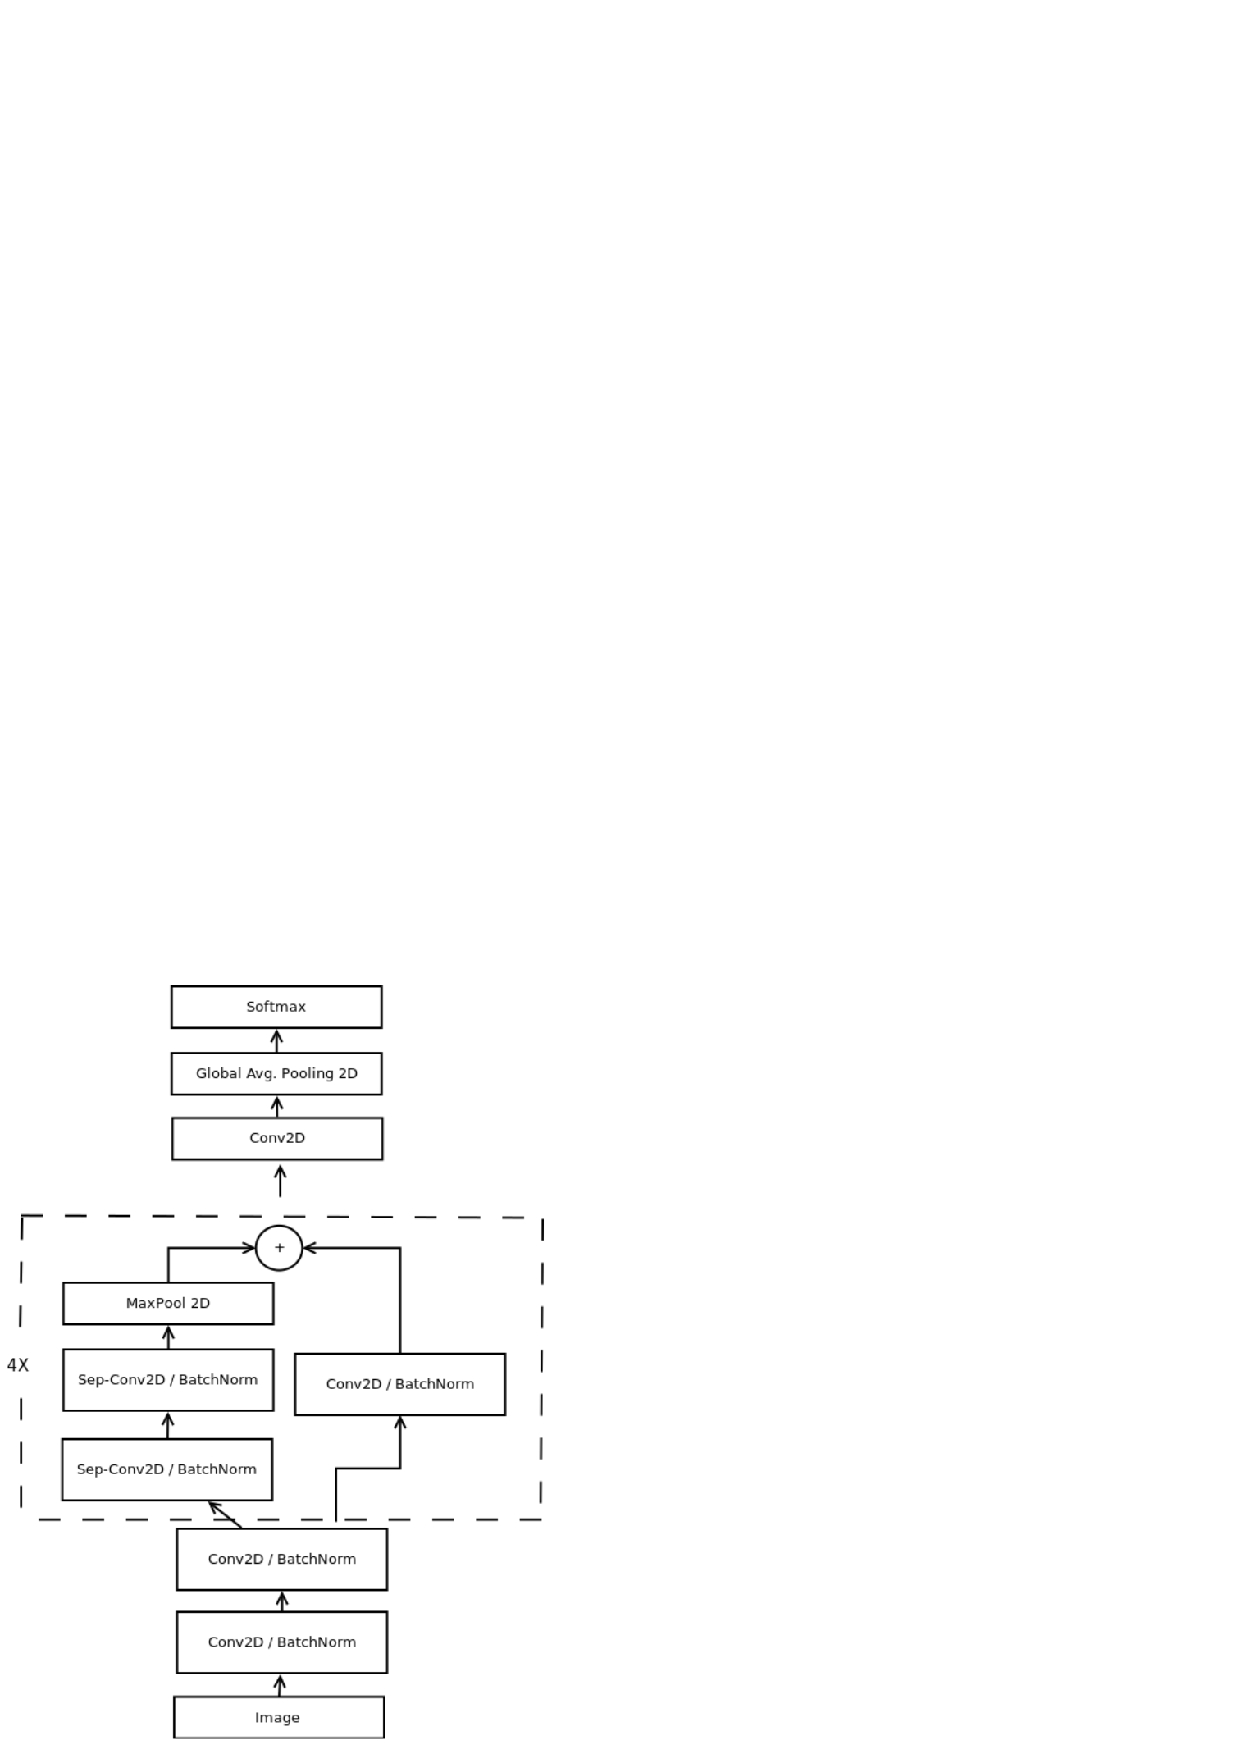
\includegraphics[scale=0.37]{Fig/cnnModel.pdf}
	\caption{\cite{Arriaga17} proposed model for real-time classification of emotions}
	\label{cnnModel}
\end{center}
\end{figure}

We used the FER-2013 emotion database, which contains 35.887 48x48 pixel grayscale labeled images. 80\% of pictures were used for training, while the remaining 20\% were used for validation of the algorithm. The achieved results were a 65\% validation accuracy accros the proposed list of emotions: (0=Angry, 1=Disgust, 2=Fear, 3=Happy, 4=Sad, 5=Surprise, 6=Neutral).

[\textbf{\emph{TODO}} - mention other results as well - like the CK+ validation result]


\chapter{Application (numerical validation)}
\label{chapter:application}

For the proposed algorithm, our approach was to perform several training sessions, with different inputs for the independent variables and see how they affect the learning. The reason for this, was to find a way to improve the accuracy of the model. As will be related in the following section, we have played around with the learning rate and with the loss function of the algorithm. Unfortunately, what we have found is that the algorithm reaches a plateou of learning from which it cannot escape, thus, the accuracy of the model being around 65\%, almost like what was achieved in \cite{Arriaga17}.

\section{Methodology}
\label{section:meth}
In this chapter, we analyze the achieved results for the proposed algorithm using the following approach. We present the training dataset and independent variables, a plot of the achieved training results and how well it fairs against the CK+ dataset, presenting the precision for each emotion separately.\\
The independent variables we are experimenting with are the learning rate, and the loss function.\\
The dependent variables will be the weights of the model.\\
For our first attempt, we have uesd the whole FER-2013 dataset, and obtained a validation accuracy of 65\%, and for the next attempts we shall only use the Training pictures from the FER-2013 dataset, and it will also enable us to compute the precision for the Public Test set nad Private Test set of the FER-2013 dataset.\\
We also compute the precision against the CK+ emotion dataset and present the results here.

\section{Obtained results}
\label{section:or}
Our \textbf{\emph{first}} trial was using the whole FER-2013 database as training, split into 80\% training and 20\% validation sets. The result was a validation accuracy of 65\%, but a model that does not fair well against the CK+ dataset at all (well, except for the happy emotion). The learning rate was 0.1 (as proposed in the paper) and the loss function was the Categorical Crossentropy.
\begin{figure}[htbp]
\begin{center}
	\includegraphics[scale=0.8]{Fig/fer_training_35k.pdf}
	\caption{Training results using all the 35.887 images in the FER-2013 emotion dataset}
	\label{fer_training_35k}
\end{center}
\end{figure}

\begin{table}[htbp]
	\caption{The precisin results against the CK+ dataset for the first training trial}
	\label{fer_training_35k_ckp}
		\begin{center}
			\begin{tabular}{p{110pt}p{110pt}c}
				\textbf{Emotion}& \textbf{Precision}& \textbf{No. of pictures} \\
				\hline\hline
				Angry& 0.16& 45 \\
				Disgust& 0.00& 59 \\
				Fear& 0.03& 25 \\
				Happy& 0.68& 69 \\
				Sad& 0.12& 28 \\
				Surprise& 0.00& 83 \\
				Neutral& 0.03& 1 \\
				\hline
				Weighted Average& 0.19
			\end{tabular}
		\end{center}
\end{table}
\pagebreak

Our \textbf{\emph{second}} attempt uses just the Training set of the FER-2013 dataset, split into 80\% training and 20\% validation sets. The result was a validation accuracy of 63\%, and a 43\% accuracy on the CK+ dataset (better ones for Happy and Surprise emotion). The learning rate was 0.1 (as proposed in the paper) and the loss function was the Categorical Crossentropy.
\begin{figure}[htbp]
\begin{center}
	\includegraphics[scale=0.8]{Fig/fer_training_28k_01.pdf}
	\caption{Training results using 28.709 images from the FER-2013 emotion dataset}
	\label{fer_training_28k_01}
\end{center}
\end{figure}

\begin{table}[htbp]
	\caption{The precisin results against the CK+ dataset for the second training trial}
	\label{fer_training_28k_01_ckp}
		\begin{center}
			\begin{tabular}{p{110pt}p{110pt}c}
				\textbf{Emotion}& \textbf{Precision}& \textbf{No. of pictures} \\
				\hline\hline
				Angry& 0.19& 45 \\
				Disgust& 0.00& 59 \\
				Fear& 0.05& 25 \\
				Happy& 0.52& 69 \\
				Sad& 0.15& 28 \\
				Surprise& 1.00& 83 \\
				Neutral& 0.00& 1 \\
				\hline
				Weighted Average& 0.43
			\end{tabular}
		\end{center}
\end{table}
\begin{table}[htbp]
	\caption{The precisin results against the FER-2013 Public Test dataset for the second training trial}
	\label{fer_training_28k_01_public_test}
		\begin{center}
			\begin{tabular}{p{110pt}p{110pt}c}
				\textbf{Emotion}& \textbf{Precision}& \textbf{No. of pictures} \\
				\hline\hline
				Angry& 0.51& 467 \\
				Disgust& 0.67& 56 \\
				Fear& 0.47& 496 \\
				Happy& 0.82& 895 \\
				Sad& 0.52& 653 \\
				Surprise& 0.74& 415 \\
				Neutral& 0.55& 607 \\
				\hline
				Weighted Average& 0.62 &3589
			\end{tabular}
		\end{center}
\end{table}
\begin{table}[htbp]
	\caption{The precisin results against the FER-2013 Private Test dataset for the second training trial}
	\label{fer_training_28k_01_private_test}
		\begin{center}
			\begin{tabular}{p{110pt}p{110pt}c}
				\textbf{Emotion}& \textbf{Precision}& \textbf{No. of pictures} \\
				\hline\hline
				Angry& 0.53& 467 \\
				Disgust& 0.47& 56 \\
				Fear& 0.47& 496 \\
				Happy& 0.84& 895 \\
				Sad& 0.50& 653 \\
				Surprise& 0.74& 415 \\
				Neutral& 0.61& 607 \\
				\hline
				Weighted Average& 0.63 &3589
			\end{tabular}
		\end{center}
\end{table}
\pagebreak

Our \textbf{\emph{third}} attempt uses just the Training set of the FER-2013 dataset, split into 80\% training and 20\% validation sets. The result was a validation accuracy of 63\%, and a 45\% accuracy on the CK+ dataset (better ones for Happy and Surprise emotion). The learning rate was 0.01 (smaller than proposed in the paper) and the loss function was the Categorical Crossentropy.
\begin{figure}[htbp]
\begin{center}
	\includegraphics[scale=0.8]{Fig/fer_training_28k_001.pdf}
	\caption{Training results using 28.709 images from the FER-2013 emotion dataset}
	\label{fer_training_28k_001}
\end{center}
\end{figure}

\begin{table}[htbp]
	\caption{The precisin results against the CK+ dataset for the second training trial}
	\label{fer_training_28k_001_ckp}
		\begin{center}
			\begin{tabular}{p{110pt}p{110pt}c}
				\textbf{Emotion}& \textbf{Precision}& \textbf{No. of pictures} \\
				\hline\hline
				Angry& 0.17& 45 \\
				Disgust& 0.00& 59 \\
				Fear& 0.02& 25 \\
				Happy& 0.62& 69 \\
				Sad& 0.18& 28 \\
				Surprise& 1.00& 83 \\
				Neutral& 0.02& 1 \\
				\hline
				Weighted Average& 0.45
			\end{tabular}
		\end{center}
\end{table}
\begin{table}[htbp]
	\caption{The precisin results against the FER-2013 Public Test dataset for the third training trial}
	\label{fer_training_28k_001_public_test}
		\begin{center}
			\begin{tabular}{p{110pt}p{110pt}c}
				\textbf{Emotion}& \textbf{Precision}& \textbf{No. of pictures} \\
				\hline\hline
				Angry& 0.52& 467 \\
				Disgust& 0.62& 56 \\
				Fear& 0.48& 496 \\
				Happy& 0.84& 895 \\
				Sad& 0.54& 653 \\
				Surprise& 0.74& 415 \\
				Neutral& 0.55& 607 \\
				\hline
				Weighted Average& 0.63 &3589
			\end{tabular}
		\end{center}
\end{table}
\begin{table}[htbp]
	\caption{The precisin results against the FER-2013 Private Test dataset for the third training trial}
	\label{fer_training_28k_001_private_test}
		\begin{center}
			\begin{tabular}{p{110pt}p{110pt}c}
				\textbf{Emotion}& \textbf{Precision}& \textbf{No. of pictures} \\
				\hline\hline
				Angry& 0.57& 467 \\
				Disgust& 0.73& 56 \\
				Fear& 0.48& 496 \\
				Happy& 0.85& 895 \\
				Sad& 0.48& 653 \\
				Surprise& 0.76& 415 \\
				Neutral& 0.59& 607 \\
				\hline
				Weighted Average& 0.64 &3589
			\end{tabular}
		\end{center}
\end{table}
\pagebreak

Seeing that our \textbf{\emph{third}} attempt was a little bit more successful than our \textbf{\emph{second}} attempt, for the \textbf{\emph{fourth}} attempt we decided to stick with the 0.01 learning rate, but to experiment with the loss function, changing it to the Mean Square Error. \\
Our \textbf{\emph{fourth}} attempt still uses just the Training set of the FER-2013 dataset, split into 80\% training and 20\% validation sets. The result were a validation accuracy of 63\%, and a 42\% accuracy on the CK+ dataset (better ones for Happy and Surprise emotion). The learning rate was 0.01 (smaller than proposed in the paper) and the loss function was the Mean Squre Error.
\begin{figure}[htbp]
\begin{center}
	\includegraphics[scale=0.8]{Fig/fer_training_28k_001_mean_square.pdf}
	\caption{Training results using 28.709 images from the FER-2013 emotion dataset}
	\label{fer_training_28k_001_mean_square}
\end{center}
\end{figure}

\begin{table}[htbp]
	\caption{The precisin results against the CK+ dataset for the fourth training trial}
	\label{fer_training_28k_001_mean_square_ckp}
		\begin{center}
			\begin{tabular}{p{110pt}p{110pt}c}
				\textbf{Emotion}& \textbf{Precision}& \textbf{No. of pictures} \\
				\hline\hline
				Angry& 0.13& 45 \\
				Disgust& 0.00& 59 \\
				Fear& 0.12& 25 \\
				Happy& 0.49& 69 \\
				Sad& 0.12& 28 \\
				Surprise& 1.00& 83 \\
				Neutral& 0.00& 1 \\
				\hline
				Weighted Average& 0.42
			\end{tabular}
		\end{center}
\end{table}
\begin{table}[htbp]
	\caption{The precisin results against the FER-2013 Public Test dataset for the fourth training trial}
	\label{fer_training_28k_001_mean_square_public_test}
		\begin{center}
			\begin{tabular}{p{110pt}p{110pt}c}
				\textbf{Emotion}& \textbf{Precision}& \textbf{No. of pictures} \\
				\hline\hline
				Angry& 0.53& 467 \\
				Disgust& 0.61& 56 \\
				Fear& 0.51& 496 \\
				Happy& 0.82& 895 \\
				Sad& 0.54& 653 \\
				Surprise& 0.76& 415 \\
				Neutral& 0.53& 607 \\
				\hline
				Weighted Average& 0.63 &3589
			\end{tabular}
		\end{center}
\end{table}
\begin{table}[htbp]
	\caption{The precisin results against the FER-2013 Private Test dataset for the fourth training trial}
	\label{fer_training_28k_001_mean_square_private_test}
		\begin{center}
			\begin{tabular}{p{110pt}p{110pt}c}
				\textbf{Emotion}& \textbf{Precision}& \textbf{No. of pictures} \\
				\hline\hline
				Angry& 0.56& 467 \\
				Disgust& 0.52& 56 \\
				Fear& 0.50& 496 \\
				Happy& 0.85& 895 \\
				Sad& 0.49& 653 \\
				Surprise& 0.74& 415 \\
				Neutral& 0.58& 607 \\
				\hline
				Weighted Average& 0.63 &3589
			\end{tabular}
		\end{center}
\end{table}
\pagebreak

Since the model did not improve with our \textbf{\emph{fourth}} attempt, we decided to give it another go, and use the same Mean Square Error, but this time with a learning rate of 0.1. \\
Out \textbf{\emph{fifth}} attempt still uses just the Training set of the FER-2013 dataset, split into 80\% training and 20\% validation sets. The result were a validation accuracy of 64\%, and a 37\% accuracy on the CK+ dataset (better ones for Happy, Surprise and Neutral emotion). The learning rate was 0.1 (as proposed in the paper) and the loss function was the Mean Squre Error.
\begin{figure}[htbp]
\begin{center}
	\includegraphics[scale=0.8]{Fig/fer_training_28k_01_mean_square.pdf}
	\caption{Training results using 28.709 images from the FER-2013 emotion dataset}
	\label{fer_training_28k_01_mean_square}
\end{center}
\end{figure}

\begin{table}[htbp]
	\caption{The precisin results against the CK+ dataset for the fifth training trial}
	\label{fer_training_28k_01_mean_square_ckp}
		\begin{center}
			\begin{tabular}{p{110pt}p{110pt}c}
				\textbf{Emotion}& \textbf{Precision}& \textbf{No. of pictures} \\
				\hline\hline
				Angry& 0.16& 45 \\
				Disgust& 0.00& 59 \\
				Fear& 0.05& 25 \\
				Happy& 0.52& 69 \\
				Sad& 0.18& 28 \\
				Surprise& 0.80& 83 \\
				Neutral& 0.80& 1 \\
				\hline
				Weighted Average& 0.37
			\end{tabular}
		\end{center}
\end{table}
\begin{table}[htbp]
	\caption{The precisin results against the FER-2013 Public Test dataset for the fifth training trial}
	\label{fer_training_28k_01_mean_square_public_test}
		\begin{center}
			\begin{tabular}{p{110pt}p{110pt}c}
				\textbf{Emotion}& \textbf{Precision}& \textbf{No. of pictures} \\
				\hline\hline
				Angry& 0.53& 467 \\
				Disgust& 0.56& 56 \\
				Fear& 0.48& 496 \\
				Happy& 0.84& 895 \\
				Sad& 0.56& 653 \\
				Surprise& 0.78& 415 \\
				Neutral& 0.53& 607 \\
				\hline
				Weighted Average& 0.63 &3589
			\end{tabular}
		\end{center}
\end{table}
\begin{table}[htbp]
	\caption{The precisin results against the FER-2013 Private Test dataset for the fifth training trial}
	\label{fer_training_28k_01_mean_square_private_test}
		\begin{center}
			\begin{tabular}{p{110pt}p{110pt}c}
				\textbf{Emotion}& \textbf{Precision}& \textbf{No. of pictures} \\
				\hline\hline
				Angry& 0.54& 467 \\
				Disgust& 0.62& 56 \\
				Fear& 0.47& 496 \\
				Happy& 0.87& 895 \\
				Sad& 0.49& 653 \\
				Surprise& 0.76& 415 \\
				Neutral& 0.58& 607 \\
				\hline
				Weighted Average& 0.64 &3589
			\end{tabular}
		\end{center}
\end{table}
\pagebreak



While the achieved results were not an improvement of the original approach proposed in \cite{Arriaga17}, we can definitely say that our efforts were not in vain. What we have gathered is that there are a few emotions that are dragging the overall average of the proposed model's accuracy. These emotions are: Disgust, Fear and Neutral.\\
When testing the model against photos from the CK+ dataset, the ones we saw that have 0\% precision, like Disgust, we have seen that the model either misinterprets Disgust for Angry, thus yielding a 0\% precision, or sometimes, the labels for those pictures is just wrong. Even the CK+ dataset description recognizes this: that the emotion labels in their dataset are the labels of what was asked from the people to perform and not what they actually performed. Could this be a possibility for the FER-2013 dataset as well? If so, this would mean that the training cannot be successful with wrongly labeled pictures.
Perhaps, a more valid dataset is needed in order to achieve true and better results.\\
Another observation could be that training with a high learning rate from the beginning may cause the model to reach a plateau much sooner. Lowering the learning rate seems to delay that.\\
Also, training with a different loss function, yielded improvements in the model later on (as in later epochs) as well, instead of stopping to learn since epoch 70-90, like with the proposed loss function. Experimentation with other different loss functions could prove useful.

\chapter{Conclusion and future work}
\label{chapter:concl}


\bibliographystyle{plain}
\bibliography{BibAll}

\end{document}

